\documentclass[a4paper]{article}

%% Language and font encodings
\usepackage[english]{babel}
\usepackage[utf8x]{inputenc}
\usepackage[T1]{fontenc}

%% Sets page size and margins
\usepackage[a4paper,top=3cm,bottom=2cm,left=3cm,right=3cm,marginparwidth=1.75cm]{geometry}

%% Useful packages
\usepackage{amsmath}
\usepackage{graphicx}
\usepackage[section]{placeins}
\usepackage{listings}
\usepackage[colorinlistoftodos]{todonotes}
\usepackage[colorlinks=true, allcolors=blue]{hyperref}

\title{SIMULATOR STUDY I: A Multimodal Dataset for Various Forms of Distracted Driving}
\author{Vishal Pallerla, Sakhitha Chowdary Kanyadhara}

\begin{document}
\maketitle
 \begin{abstract}
 The goal is to see how driving of people get effected in different driving conditions like No Distraction(ND), Cognitive Distraction(CD), Emotional Distraction(ED), Sensorimotor Distraction(MD) by observing and recording various explanatory variables perinasal EDA, palm EDA, Heart-rate, Breath-rate,and response variables like speed, acceleration, brake force, steering, and lane position for each of the driving modes. This is done by plotting Heart-rate(HR), Breath-rate(BR), perinasal EDA(pp), Palm EDA Signal(PEDA), Performance Response Variables(res) across time for all subjects in each driving mode.
 \end{abstract}

\section{Introduction}
This multimodal dataset was acquired in a controlled experiment on a driving simulator. The set includes data for n=68 volunteers that drove the same highway. During the experimental drives key response variables and several explanatory variables were continuously recorded. The response variables included speed, acceleration, brake force, steering, and lane position signals, while the explanatory variables included perinasal EDA, palm EDA, heart rate, breathing rate, and facial expression signals; biographical and psychometric covariates were also obtained.\\
The entire process includes finding relevant signal files for each driving mode from all the folders, then plotting them across time separately. This is for raw data. Then comes cleaning where we find the signals which have atleast one value outside the ranges defined for them and discard those signals while plotting.


\section{Data Exploration}
By Observing the structure of the files, it is as follows:
Subject->Driving Modes-> Signals
\begin{lstlisting}[language=R]
Eg: Statistical Methods\Stat\T001\5 CD\ T001-005.HR
We used file name format(Txxx-SESSION_CODE.dat where xxx stands
for the subject number and SESSION_CODE holds the acronym of the
experimental session) for finding relevant files of a particular session
in driving mode.

fileNamesPD<-list.files(recursive = T, pattern=paste("\\-00",t,".res","$",sep = ""))
So this gets the res files for all the driving modes when different values
of t are given. For t=2, res files for all subjects from PD are extracted
and saved into fileNamesPD.
Similarly, for t = 1 (BL)
	   for t = 3 (RD)
	   for t = 4 (CD)
	   for t = 5 (ED)
	   for t = 6 (MD)
	   for t = 7 (ND)
	   for t = 8 (FD)
\end{lstlisting}


\subsection{PP(Perinasal EDA Signal)}

The value of the perinasal EDA signal at time [in ∘C2], and its smoothed over value i.e Noise Reduction (NR) Perinasal EDA signal [also in ∘C2] is given. This data is already cleaned and hence we plotted the pp signal values across time. Number of signals that got plotted are as follows for each driving session.

\begin{figure}[!h]
\centering
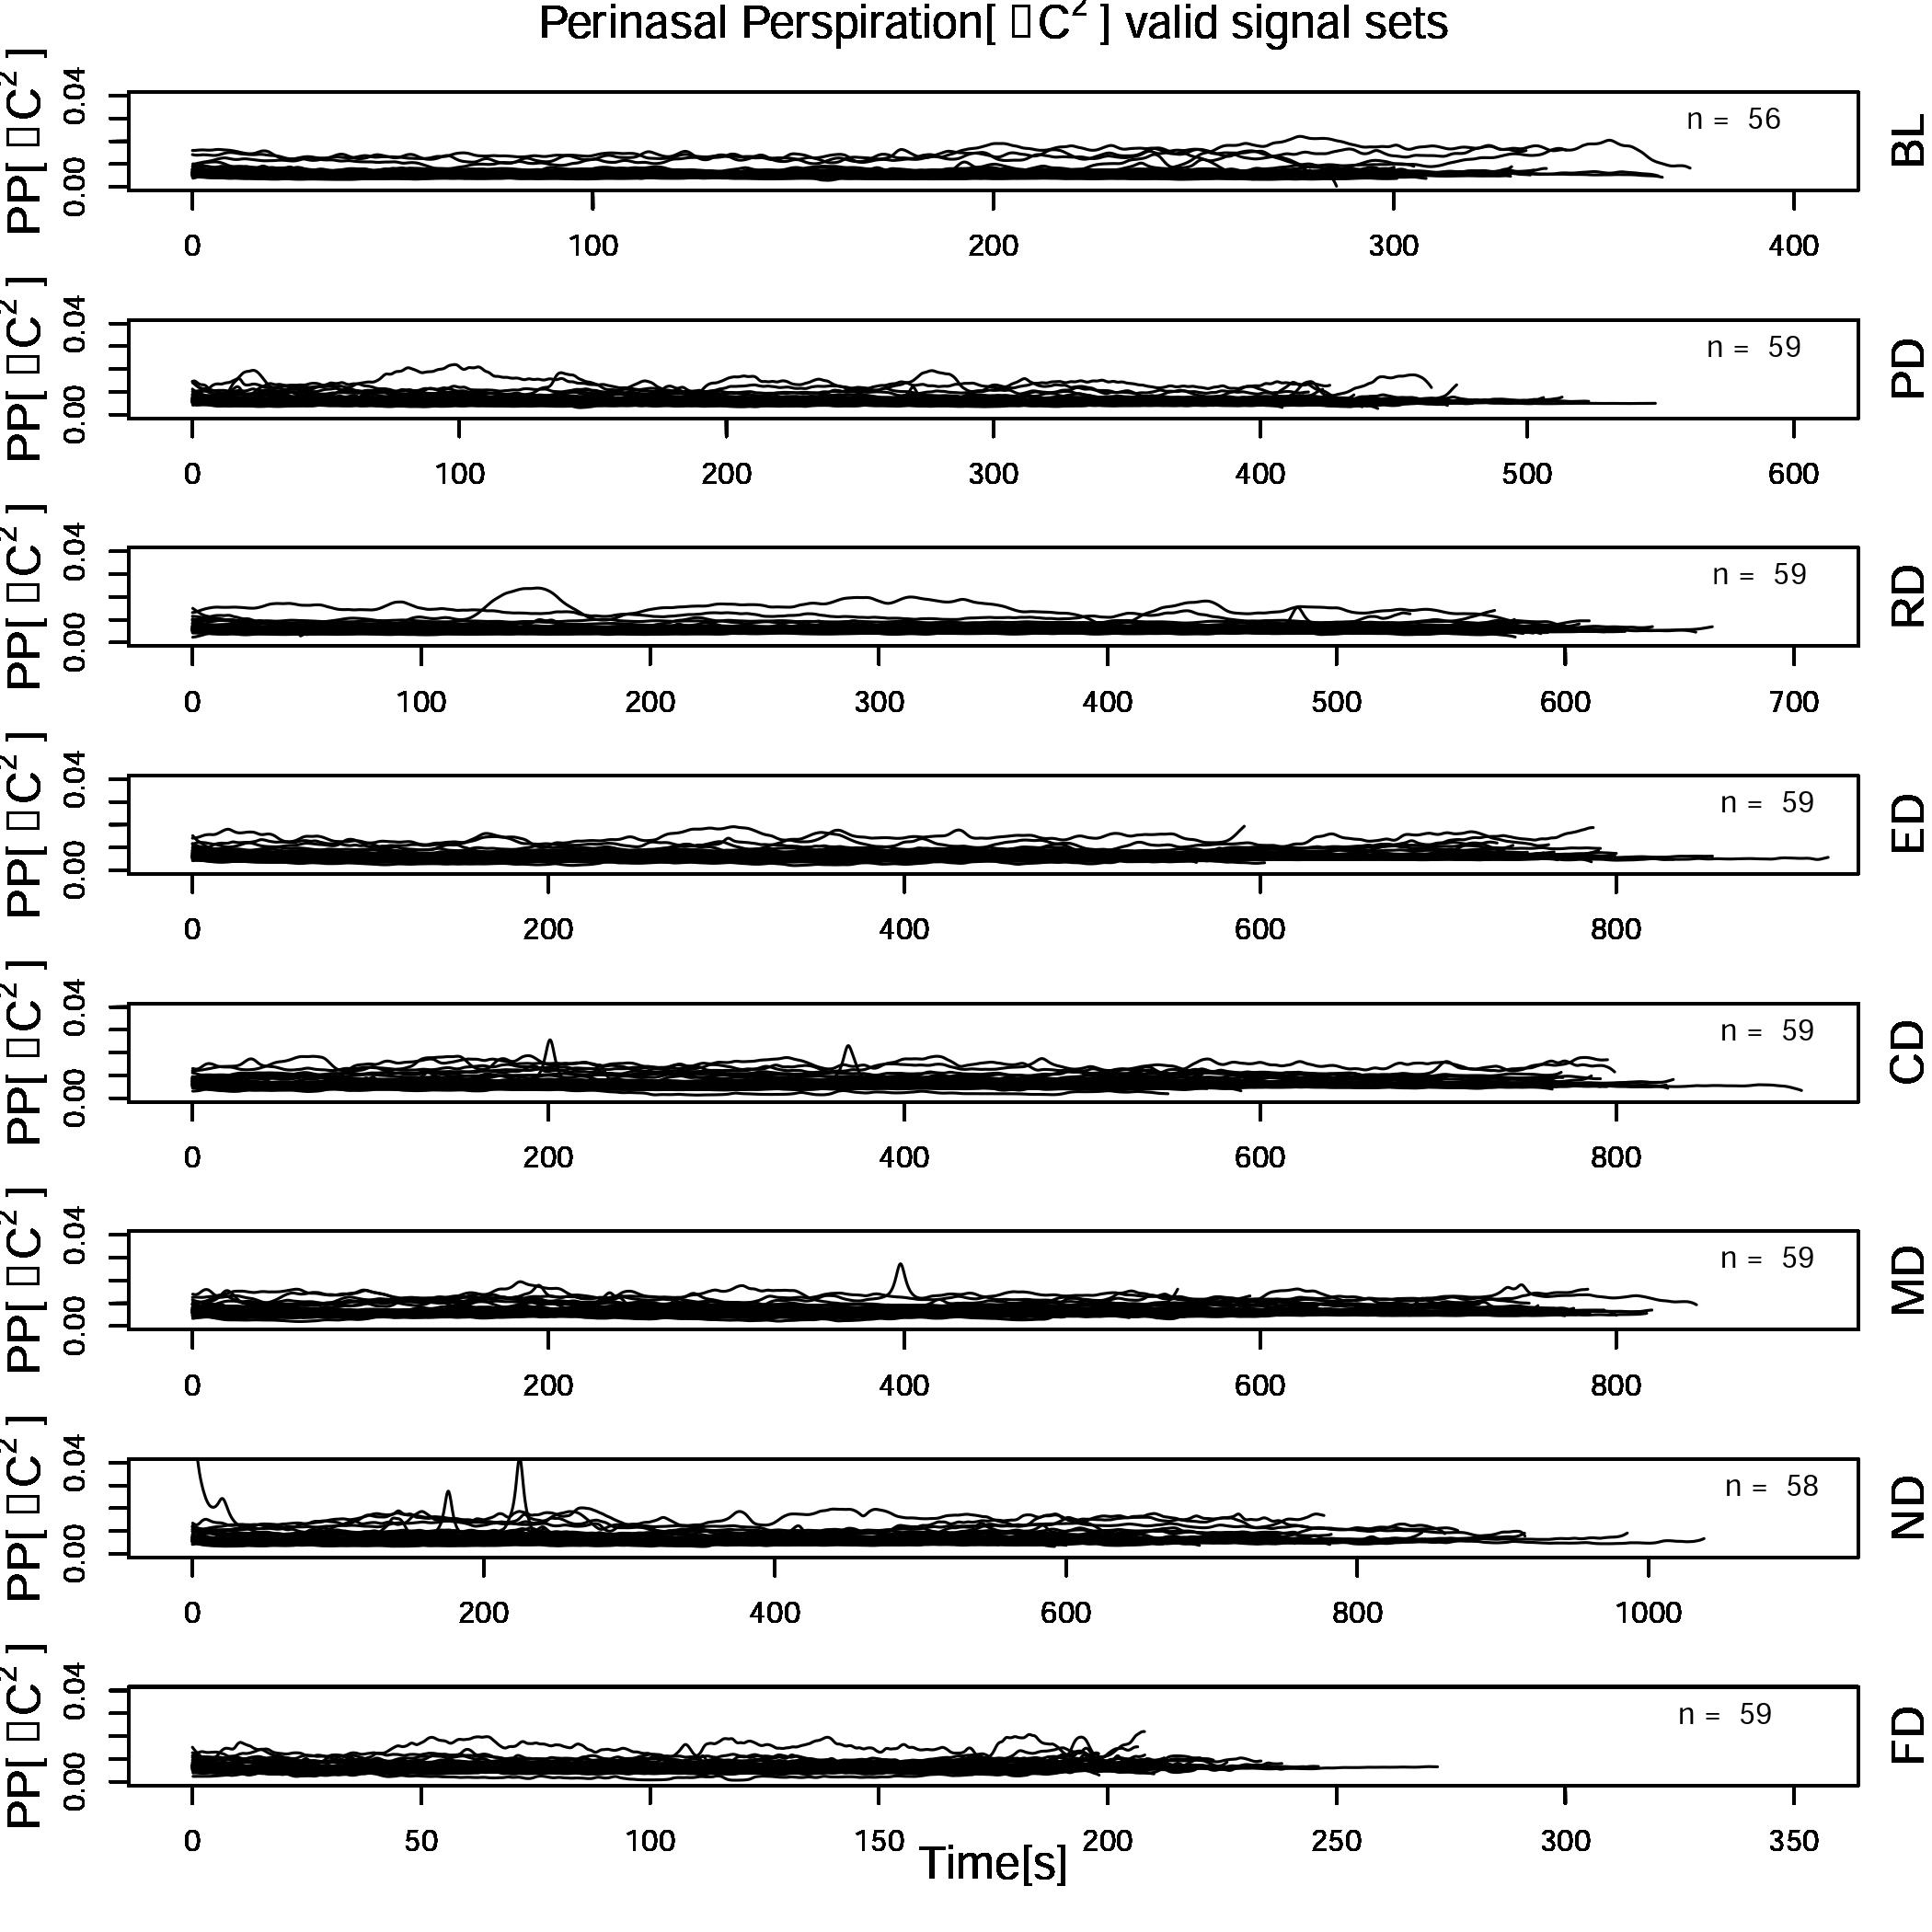
\includegraphics[width=1.0\textwidth]{pp.jpg}
\caption{\label{fig:pp}Perinasal NR EDA Signals per drive, for all subjects}
\end{figure}
\FloatBarrier
\begin{table}[!h]
\centering
\begin{tabular}{l|l}
Mode&Valid Signals\\\
BL & 56\\
PD & 59 \\
RD & 59\\
CD & 59\\
ED & 59\\
MD & 59\\
ND & 58\\
FD & 59
\end{tabular}
\caption{\label{tab:pp}Perinasal EDA Signal}
\end{table}
\FloatBarrier
\subsection{Heart Rate Signal(HR)}


It contains three columns: Frame ; Time; and Heart Rate signal.  
Process:\\
Installing the required libraries such as rJava, xlsx, openxlsx, varhandle, dplyr and calling them before use\\
library(rJava)
library(xlsx)
library(openxlsx)
library(varhandle)
library(dplyr)\\
Defined a function  with ‘t’ as a parameter where t determines the driving mode based on the number as specified in data exploration part.\\
Then all the files with extension ‘.HR’ for a driving mode are taken into a list as follows:
\begin{lstlisting}[language=R]

fileNamesPD<-list.files(recursive = T,pattern=paste("\\-00",t,".HR","$",sep = ""))
Then the raw graphs of HR are plotted using plot function and lines function.
plot(time,hr,type='l', ylab="",xlab="")
lines(time,hr,type="l")
\end{lstlisting}
Cleaning:
Raw data consisted of some HR signals which are outside the nominal range i.e (40,120) bpm, so our noise reduction algorithm uses filter from dplyr library to consider signals which are in the range and remove signals featuring at least one value outside the valid range. Only the signals that are in the range are plotted over time(s) and these set of signals are valid HR signal sets.
Discarded signals are saved in a text file named HRDiscarded.txt
Discarded Signals are:
T001/2 PD/T001-002.HR\\ 
T009/2 PD/T009-002.HR\\
T012/2 PD/T012-002.HR\\
T015/2 PD/T015-002.HR\\
T041/2 PD/T041-002.HR\\
T062/2 PD/T062-002.HR\\
T074/2 PD/T074-002.HR\\
T006/3 RD/T006-003.HR\\
T009/3 RD/T009-003.HR\\
T012/3 RD/T012-003.HR\\
T015/3 RD/T015-003.HR\\
T041/3 RD/T041-003.HR\\
T074/3 RD/T074-003.HR\\
T001/4 ND/T001-004.HR\\
T006/4 ND/T006-004.HR\\
T009/6 ND/T009-004.HR\\
T012/7 ND/T012-004.HR\\
T015/6 ND/T015-004.HR\\
T041/6 ND/T041-004.HR\\
T064/5 ND/T064-004.HR\\
T074/7 ND/T074-004.HR\\
T001/5 CD/T001-005.HR\\
T009/4 CD/T009-005.HR\\
T012/4 CD/T012-005.HR\\
T015/5 CD/T015-005.HR\\
T041/7 CD/T041-005.HR\\
T062/5 CD/T062-005.HR\\
T064/7 CD/T064-005.HR\\
T074/5 CD/T074-005.HR\\
T001/6 ED/T001-006.HR\\
T009/5 ED/T009-006.HR\\
T012/6 ED/T012-006.HR\\
T015/4 ED/T015-006.HR\\
T041/4 ED/T041-006.HR\\
T064/6 ED/T064-006.HR\\
T074/4 ED/T074-006.HR\\
T001/7 MD/T001-007.HR\\
T009/7 MD/T009-007.HR\\
T012/5 MD/T012-007.HR\\
T015/7 MD/T015-007.HR\\
T041/5 MD/T041-007.HR\\
T074/6 MD/T074-007.HR\\
T001/8 FDN/T001-008.HR\\
T009/8 FDN/T009-008.HR\\
T012/8 FDL/T012-008.HR\\
T015/8 FDN/T015-008.HR\\
T041/8 FDL/T041-008.HR\\
T064/8 FDN/T064-008.HR\\
T074/8 FDL/T074-008.HR\\
\begin{figure}[!h]
\centering
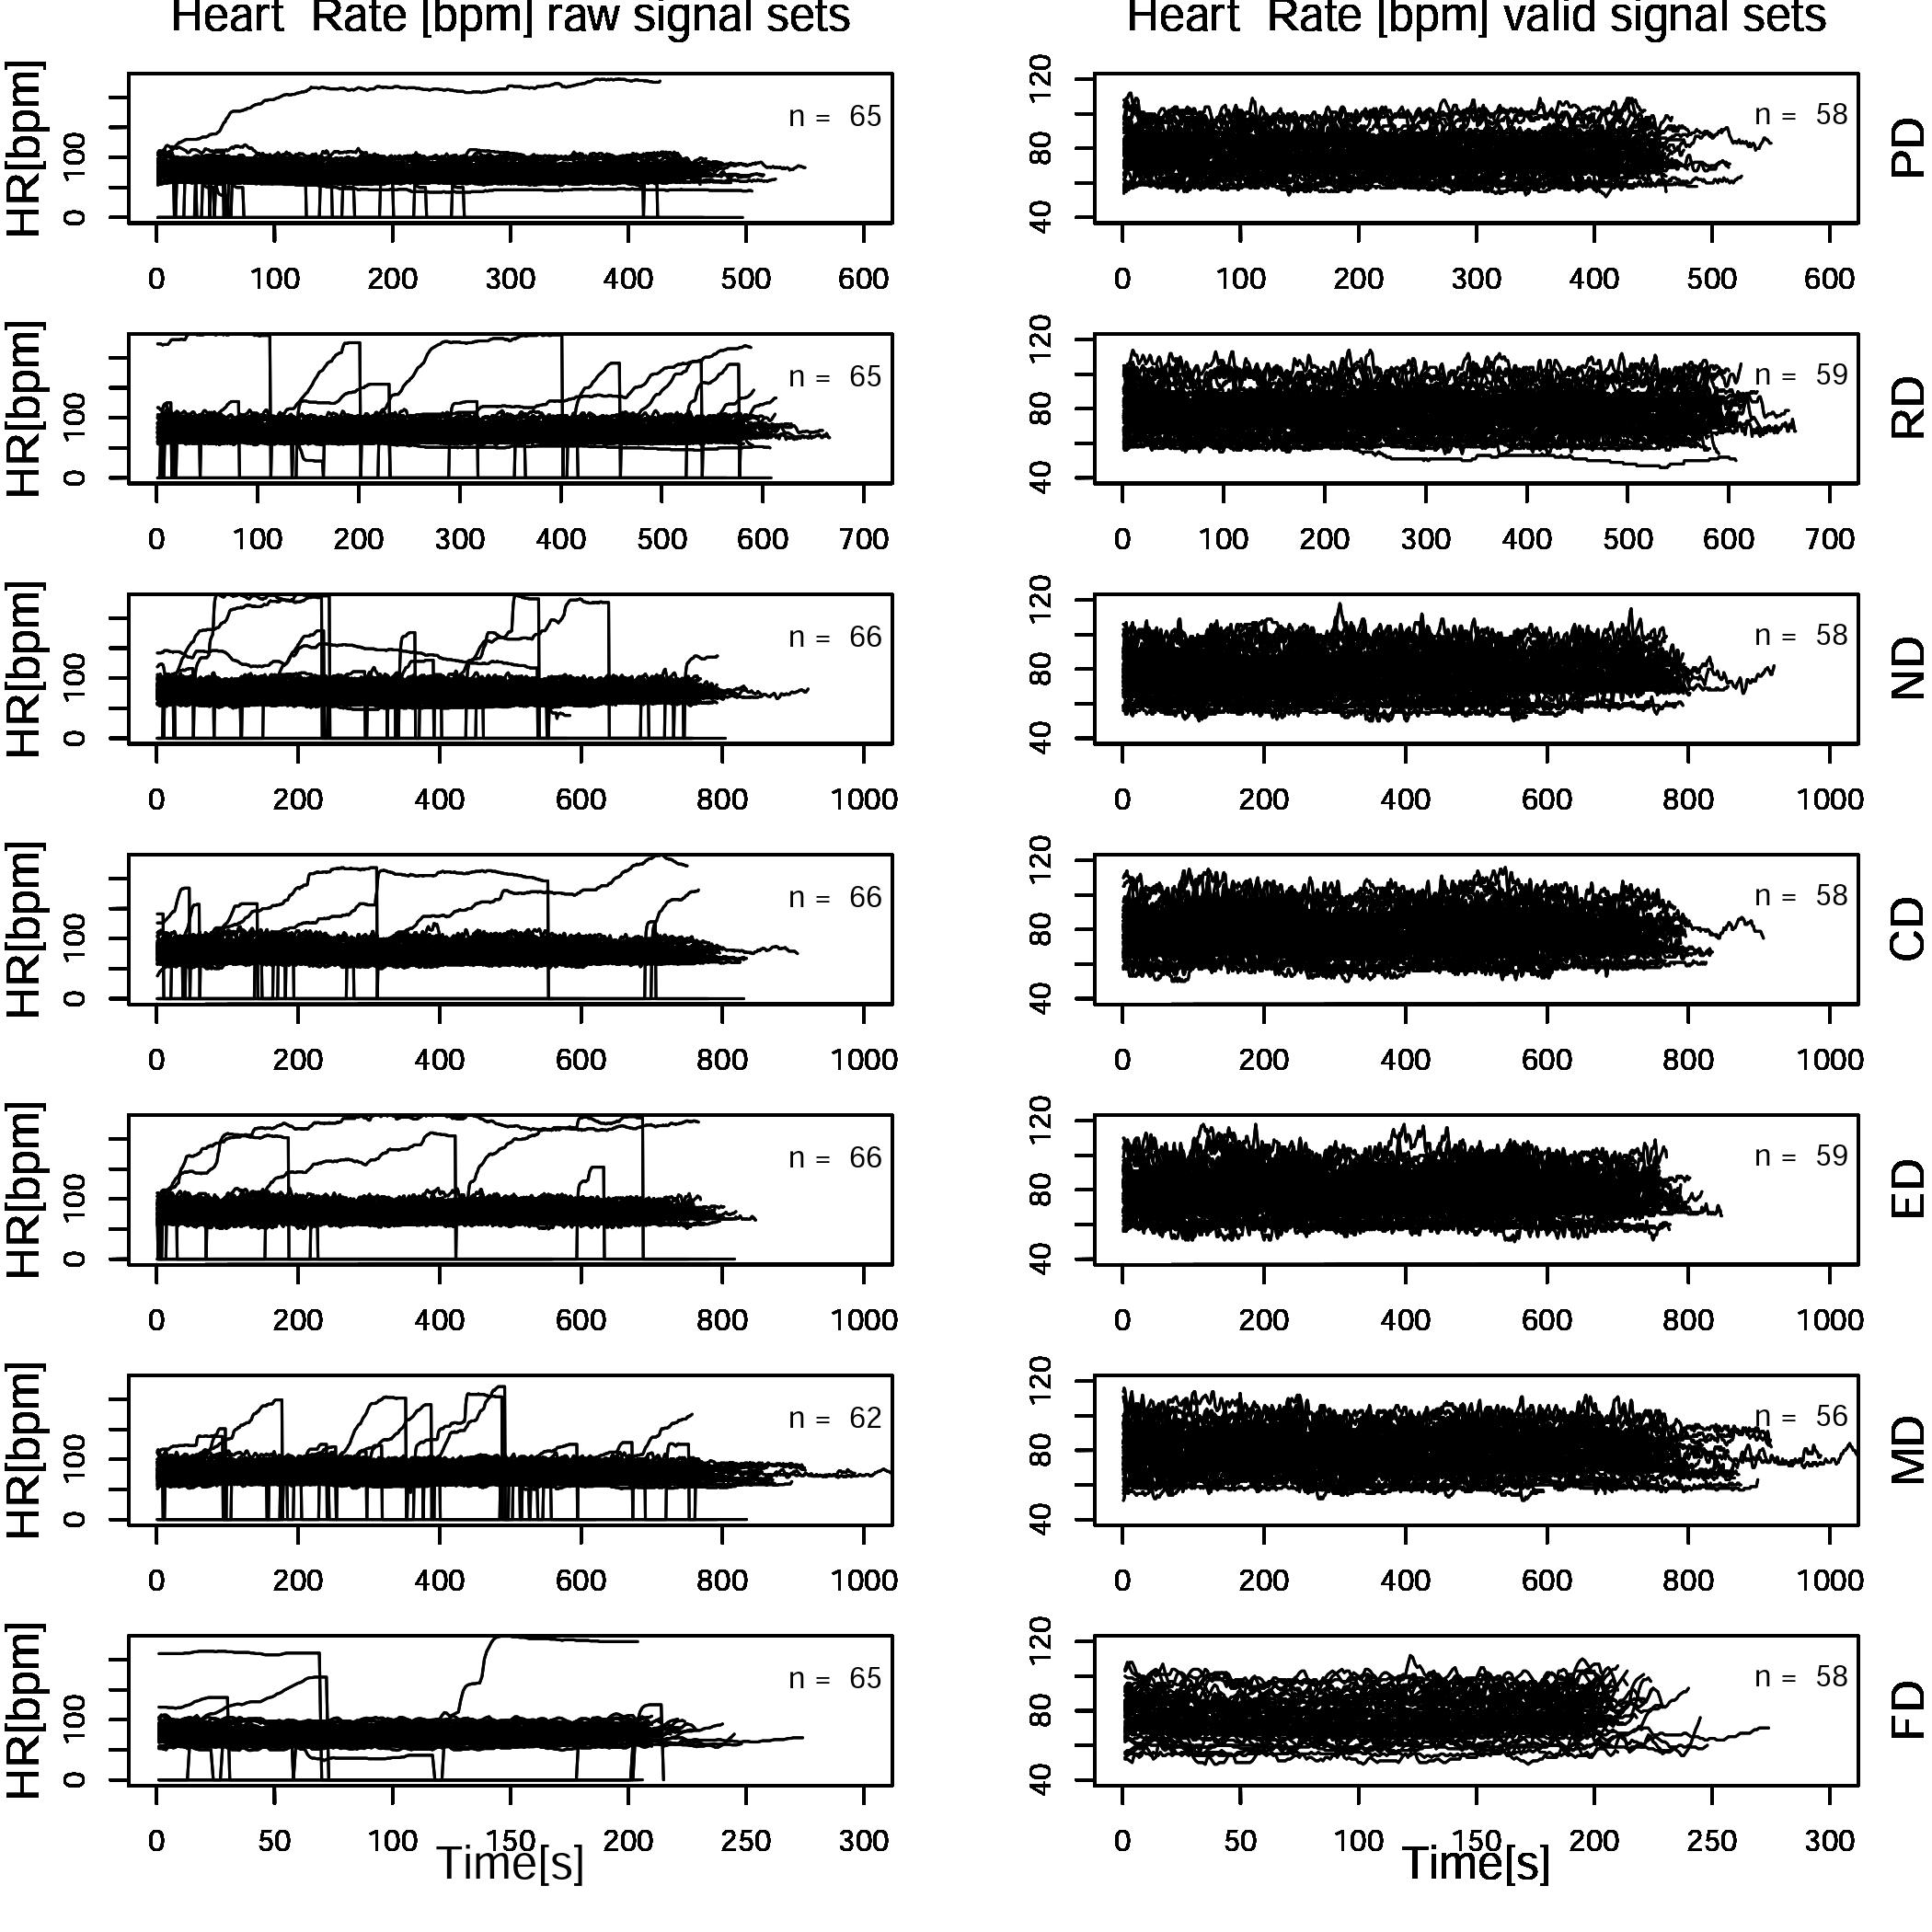
\includegraphics[width=1.0\textwidth]{hr.jpg}
\caption{\label{fig:hr}Heart Rate Signals per drive, for all subjects, before and after noise reduction-raw and valid signal sets respectively}
\end{figure}
\FloatBarrier
\begin{table}[!h]
\centering
\begin{tabular}{l|l|r}
Session & Raw Data & Valid Data \\\hline
 PD & 65 & 58 \\
RD & 65 & 59 \\
ND & 66 & 58 \\
CD & 66 & 58 \\
ED & 66 & 59 \\
MD & 62 & 56 \\
FD & 65 & 58 
 
 \end{tabular}
 \caption{\label{tab:hr}HR Raw and Valid signals}
 \end{table}

\FloatBarrier
\subsection{Breathing Rate Signal(BR)}


It contains three columns: Frame ; Time; and Breathing Rate signal.  
Syntax for installation: install.packages(rJava).
Syntax for calling: 
library(rJava)
library(xlsx)
library(openxlsx)
library(varhandle)
library(dplyr)
Defined a function  with ‘t’ as a parameter where t determines the driving mode based on the number as specified in data exploration part.
Then all the files with extension ‘.BR’ for a driving mode are taken into a list as follows:

\begin{lstlisting}[language=R]

fileNamesPD<-list.files(recursive = T,pattern=paste("\\-00",t,".BR","$",sep = ""))
Then the raw graphs of BR are plotted using plot function and lines function.
plot(time,hr,type='l', ylab="",xlab="")
lines(time,hr,type="l")
\end{lstlisting}

Cleaning:\\
Raw data consisted of some BR signals which are outside the nominal range i.e (4,70) bpm, so our noise reduction algorithm uses filter from dplyr library to consider signals which are in the range and remove signals featuring at least one value outside the valid range. Only the signals that are in the range are plotted over time(s) and these set of signals are valid BR signal sets.\\
Discarded signals are saved in a text file named BRDiscarded.txt\\
T054/5 CD/T054-005.BR\\
\begin{figure}[!h]
\centering
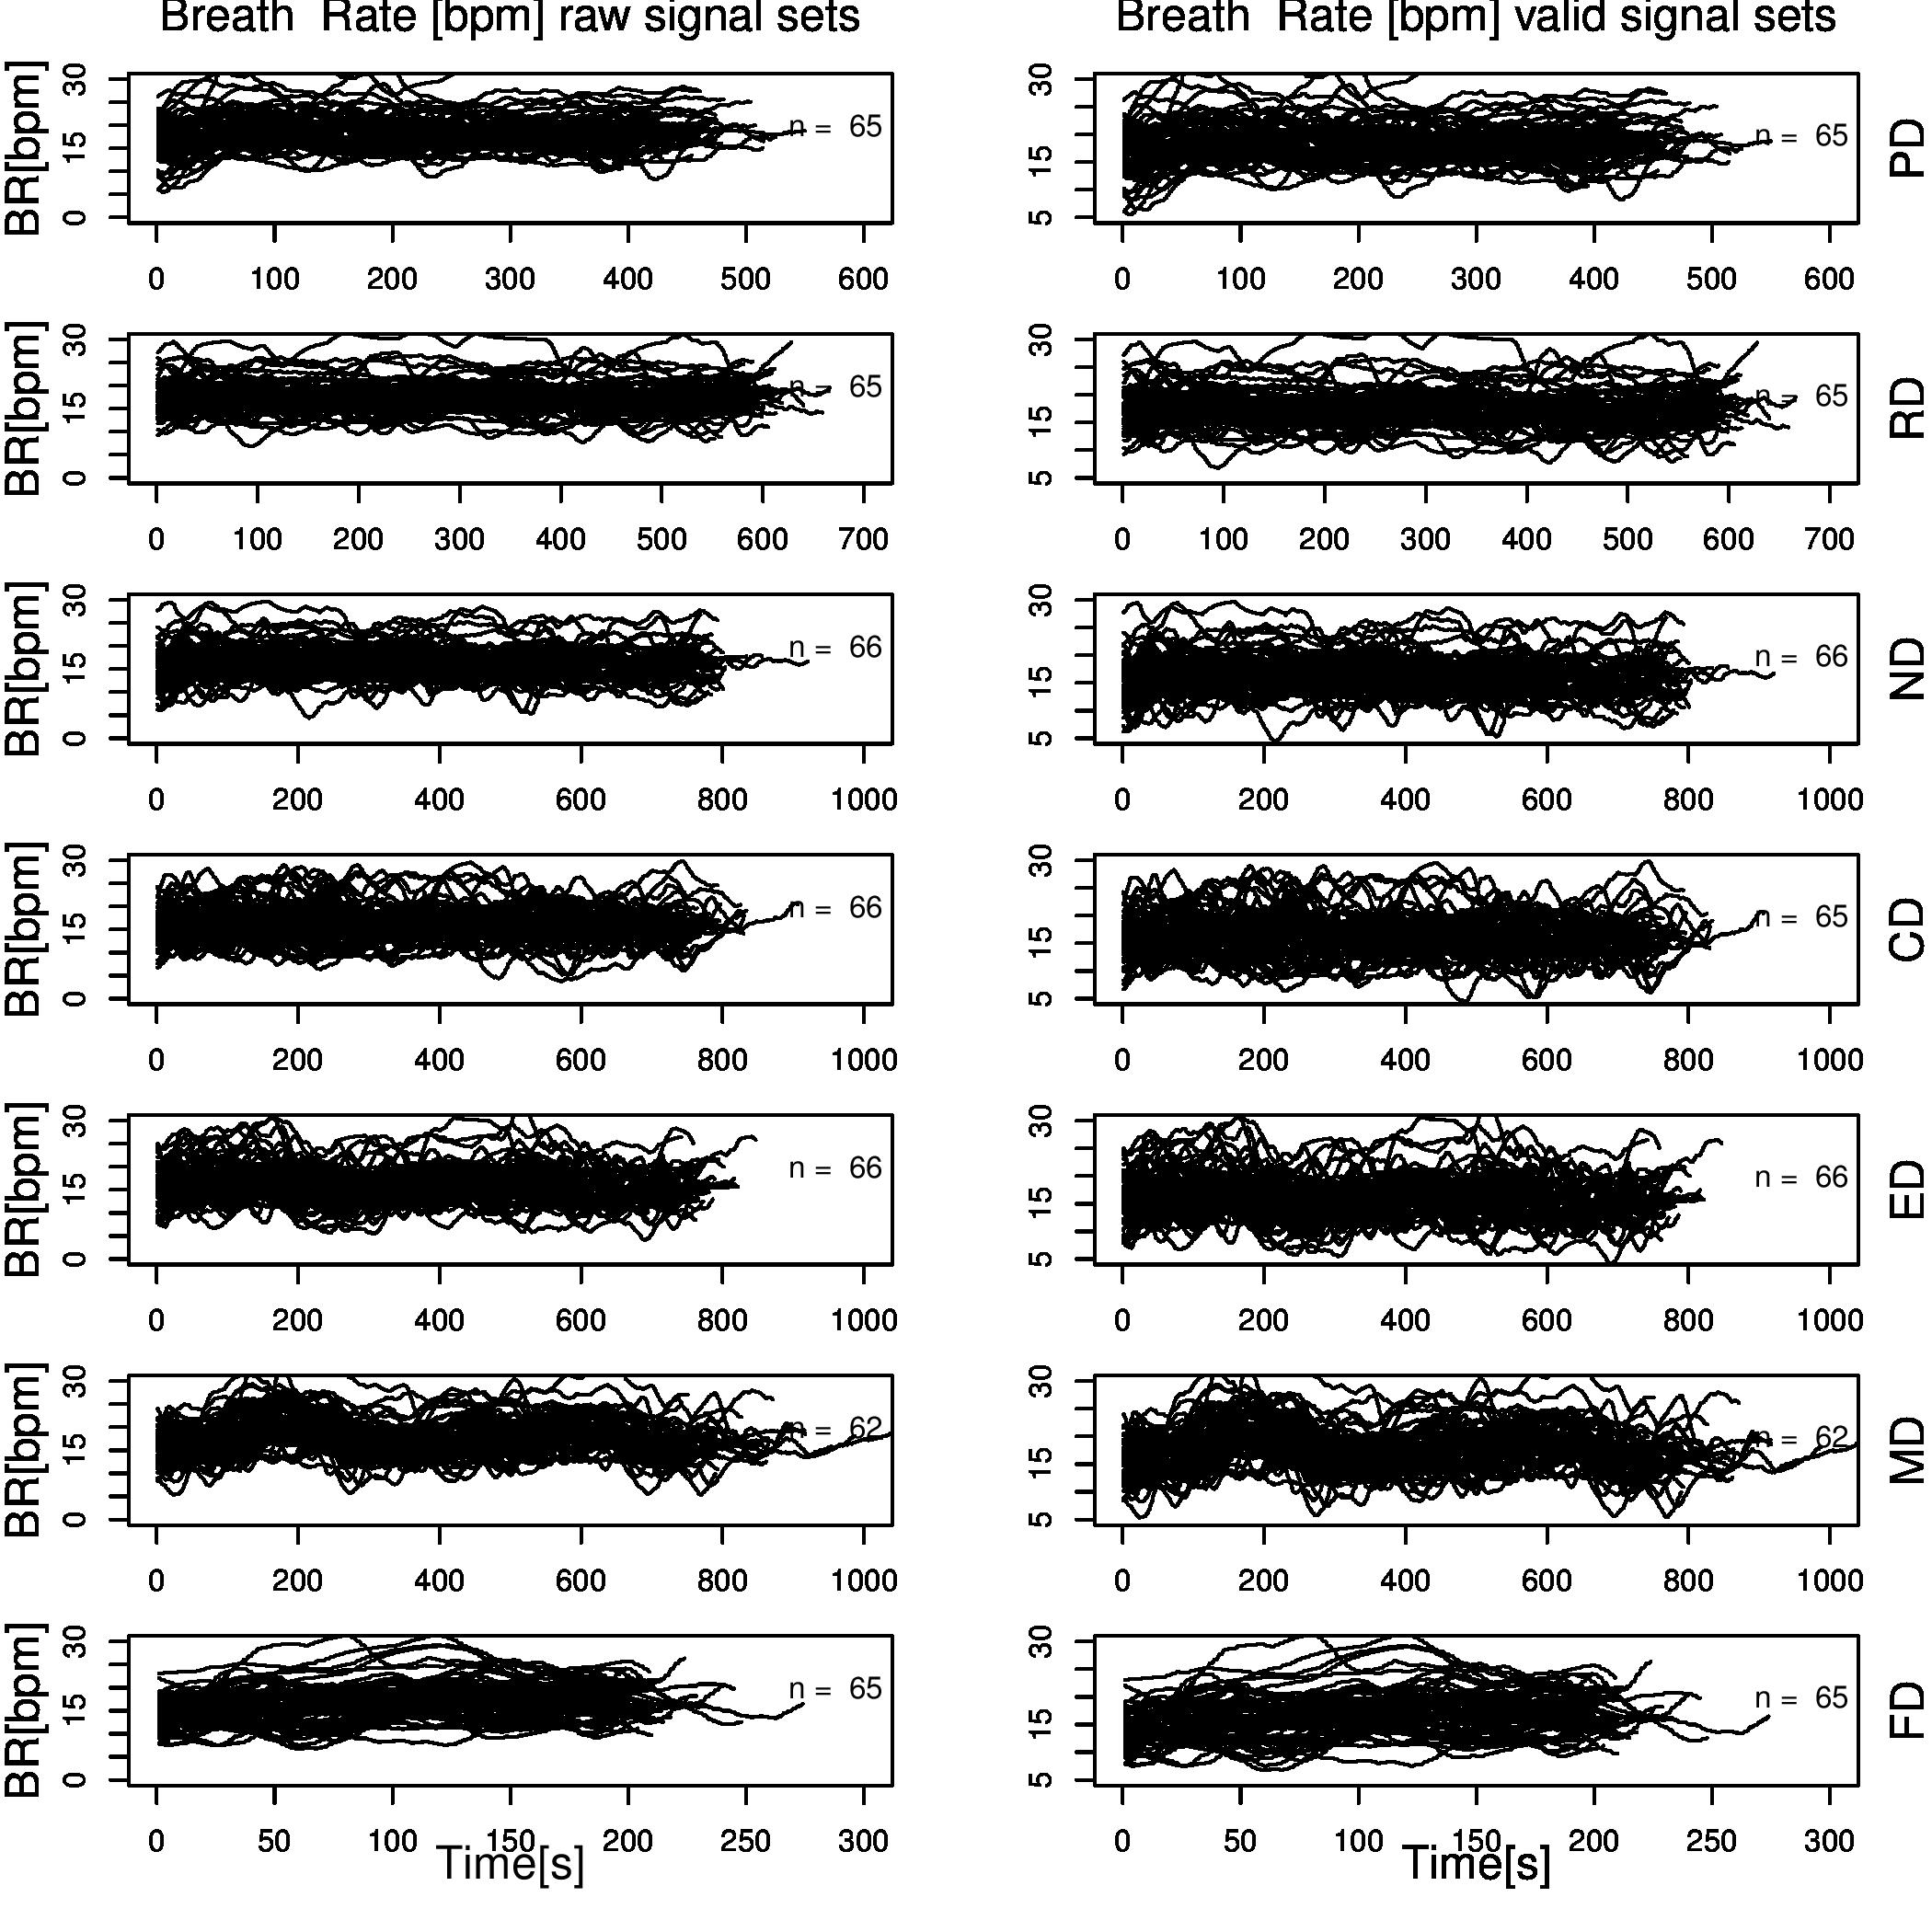
\includegraphics[width=1.0\textwidth]{BR_Raw_Clean-page-001.jpg}
\caption{\label{fig:br}Breathing Rate Signals per drive, for all subjects, before and after noise reduction-raw and valid signal sets respectively}
\end{figure}

 \begin{table}[!h]
 \centering
 \begin{tabular}{l|l|l}
Session & Raw Data & Valid Data \\\hline
 PD & 65 & 65\\
RD & 65 & 65 \\
ND & 66 & 66 \\
CD & 66 & 65 \\
ED & 66 & 66 \\
MD & 62 & 62 \\
FD & 65 & 65 
 \end{tabular}
\caption{\label{tab:br}Breathing Rate Raw and Valid Signals}
\end{table}

\FloatBarrier

\subsection{Palm EDA Signal(PEDA)}

It contains three columns: Frame ; Time; and Palm EDA signal.  \\
Process\\
Installing the required libraries such as rJava, xlsx, openxlsx, varhandle, dplyr and calling them before use\\
Syntax for installation: install.packages(rJava)\\
Syntax for calling: \\
library(rJava)\\
library(xlsx)\\
library(openxlsx)\\
library(varhandle)\\
library(dplyr)\\
Defined a function with ‘t’ as a parameter where t determines the driving mode based on the number as specified in data exploration part.\\
Then all the files with extension ‘.peda’ for a driving mode are taken into a list as follows:
\begin{lstlisting}[language=R]

fileNamesPD<-list.files(recursive = T,pattern=paste("\\-00",t,".peda","$",sep = ""))
Then the raw graphs of peda are plotted using plot function and lines function.
plot(time,hr,type='l', ylab="",xlab="")
lines(time,hr,type="l")
\end{lstlisting}
Cleaning:\\
Raw data consisted of some PEDA signals which are outside the nominal range i.e (10-4700) Kohm, so our noise reduction algorithm uses filter from dplyr library to consider signals which are in the range and remove signals featuring at least one value outside the valid range. Only the signals that are in the range are plotted over time(s) and these set of signals are valid PEDA signal sets.\\
Discarded signals are saved in a text file named PEDADiscarded.txt\\

T035/2 PD/T035-002.peda\\
T035/3 RD/T035-003.peda\\
T055/3 RD/T055-003.peda\\
T035/6 ND/T035-004.peda\\
T041/6 ND/T041-004.peda\\
T055/4 ND/T055-004.peda\\
T035/4 CD/T035-005.peda\\
T035/7 ED/T035-006.peda\\
T041/4 ED/T041-006.peda\\
T055/5 ED/T055-006.peda\\
T025/7 MD/T025-007.peda\\
T035/5 MD/T035-007.peda\\
T025/8 FDL/T025-008.peda\\
T035/8 FDL/T035-008.peda\\

\begin{figure}[h]
\centering
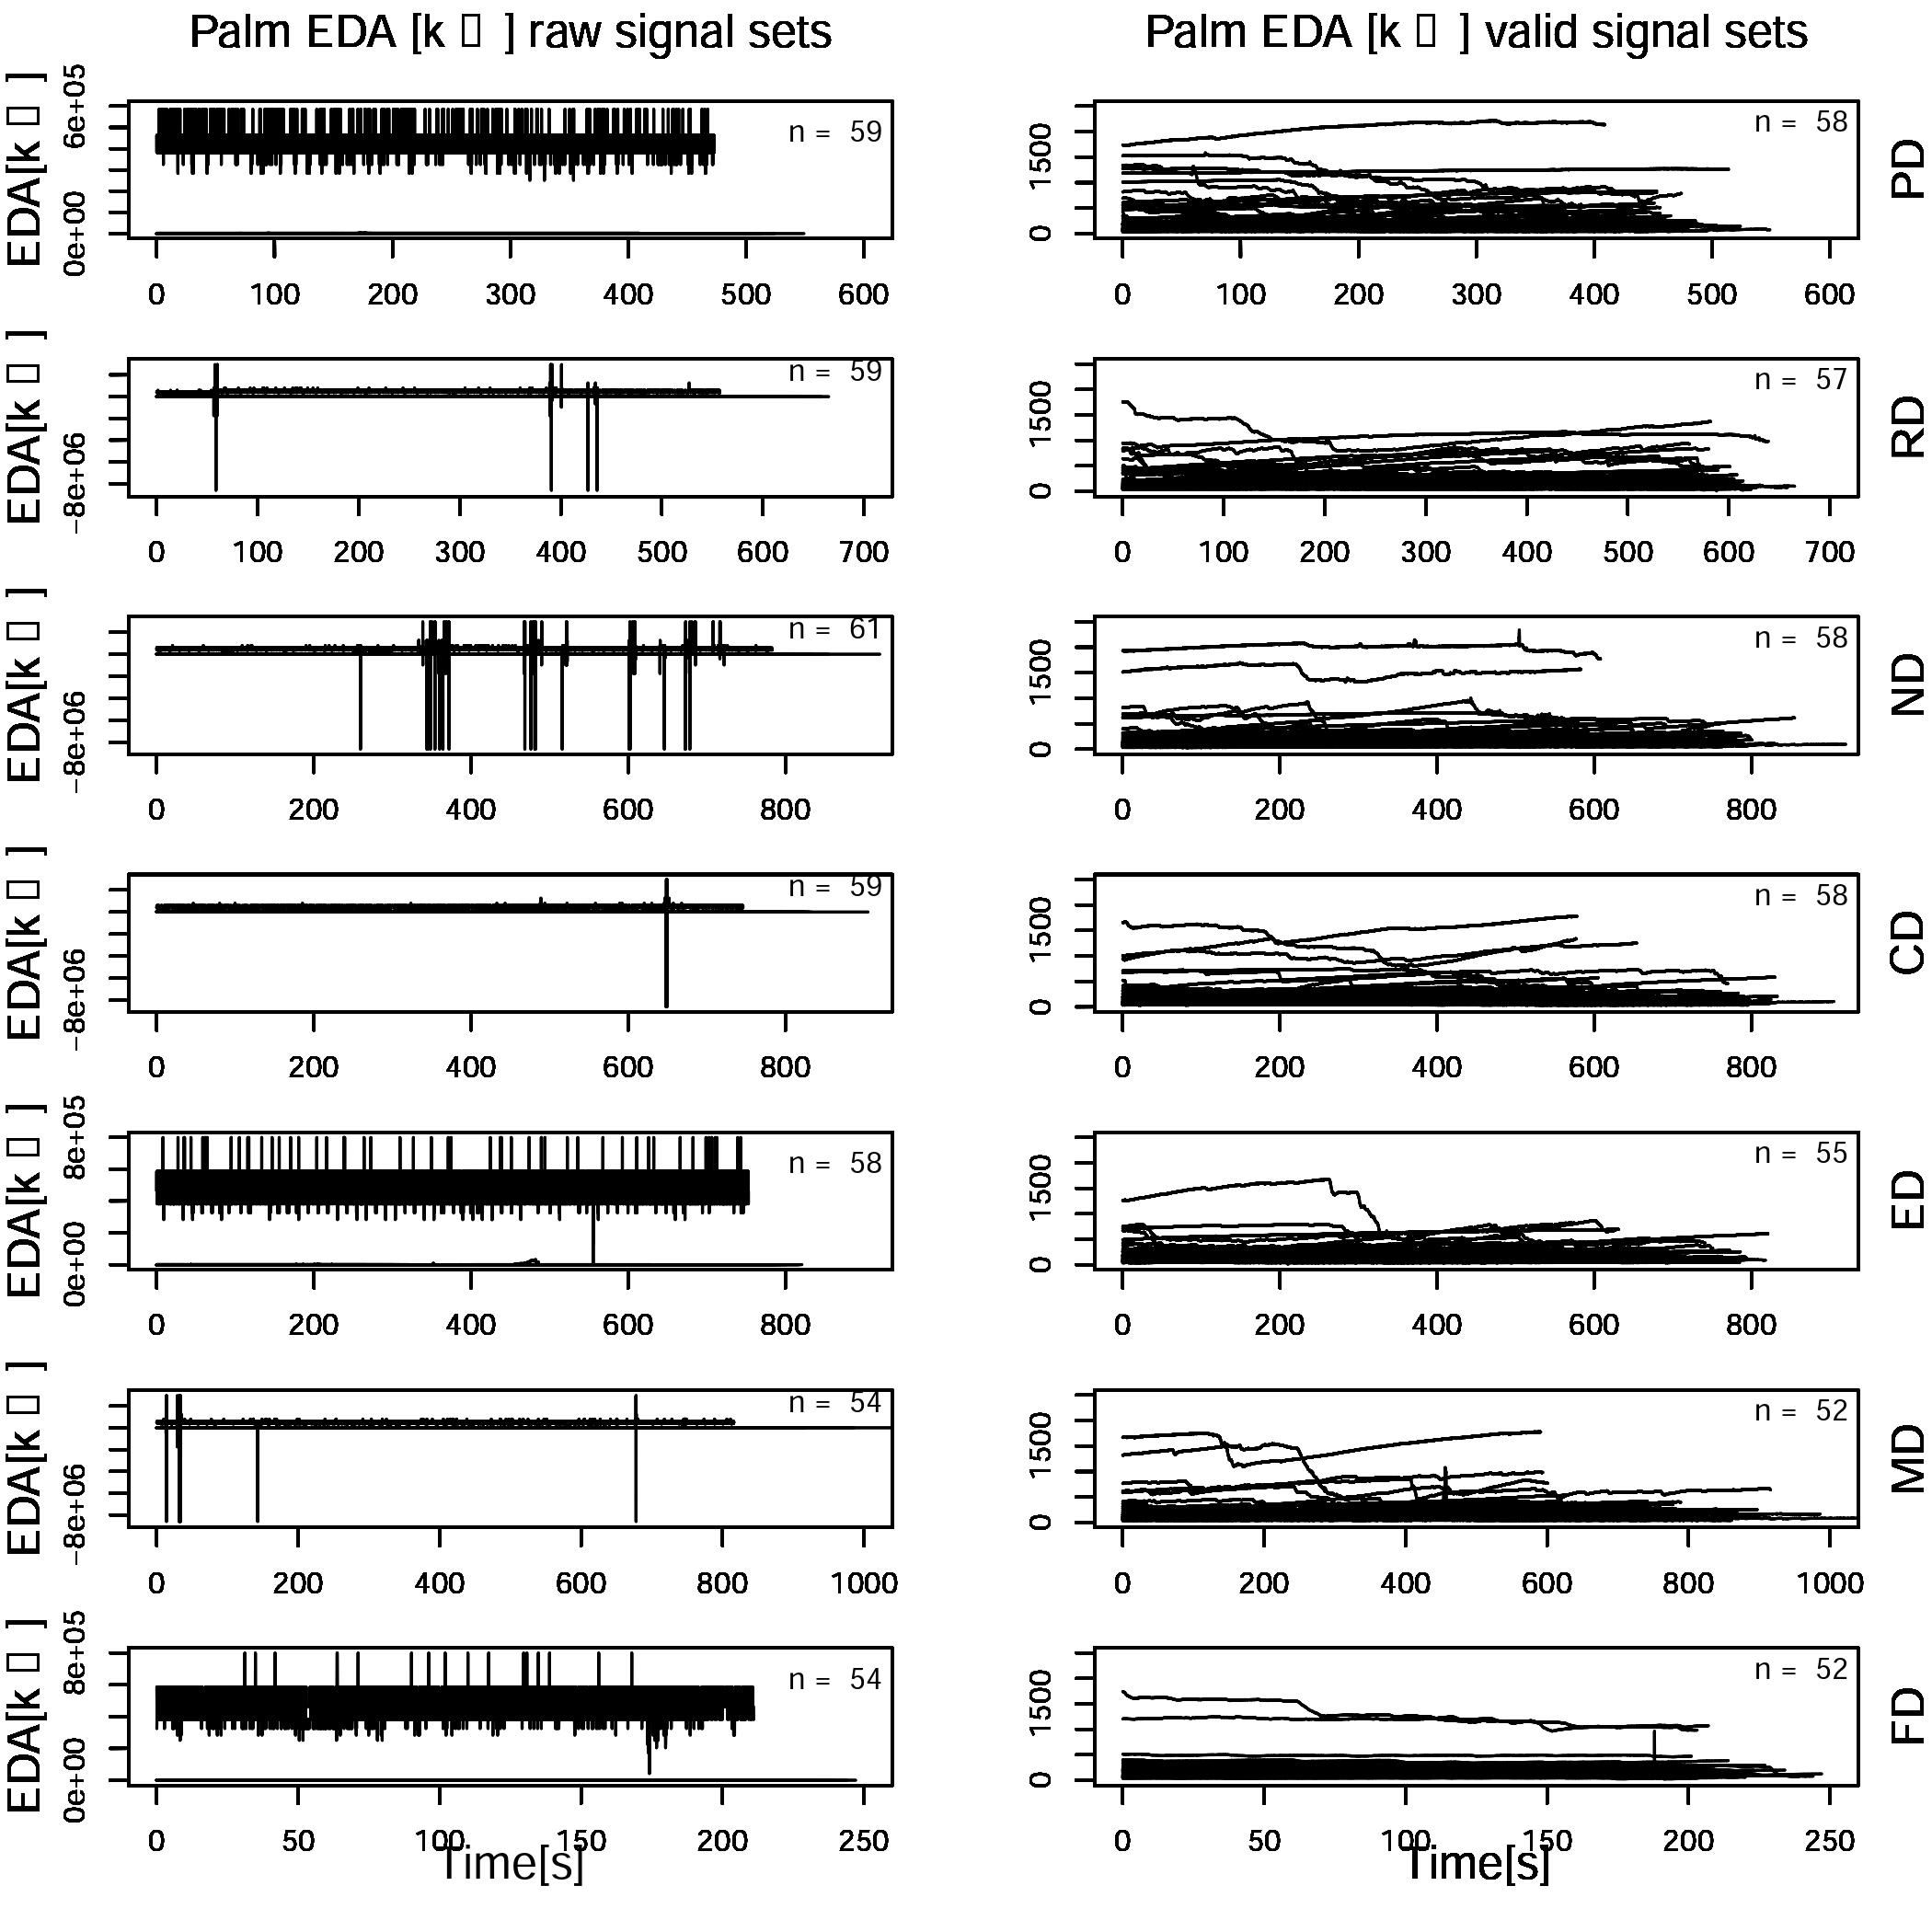
\includegraphics[width=1.0\textwidth]{peda.jpg}
\caption{\label{fig:peda}Palm EDA Signals per drive, for all subjects, before and after noise reduction-raw and valid signal sets respectively}
\end{figure}

 \begin{table}[!h]
 \centering
 \begin{tabular}{l|l|l}
Session & Raw Data & Valid Data \\\hline
 PD & 59 & 58\\
RD & 59 & 57\\
ND & 61 & 58 \\
CD & 59 & 58 \\
ED & 58 & 55 \\
MD & 54 & 52 \\
FD & 54 & 52 
 \end{tabular}
\caption{\label{tab:peda}PEDA Raw and Valid Signals}
\end{table}

\FloatBarrier

\subsection{Performance Response Variables(RES)}

 It contains Frame; Time; Speed signal; Acceleration signal; Brake Force signal; Steering signal; and, Lane Position signal.\\
Process\\
Installing the required libraries such as rJava, xlsx, openxlsx, varhandle, dplyr and calling them before use\\
Syntax for installation: install.packages(rJava)\\
Syntax for calling: \\
library(rJava)\\
library(xlsx)\\
library(openxlsx)\\
library(varhandle)\\
library(dplyr)\\
Defined  functions for speed, acceleration, breaking, steering and lane position with ‘t’ as a parameter where t determines the driving mode based on the number as specified in data exploration part.\\
Then all the files with extension ‘.res’ for a driving mode are taken into a list as follows:
\begin{lstlisting}[language=R]

fileNamesPD<-list.files(recursive = T,pattern=paste("\\-00",t,".res","$",sep = ""))
Then the raw graphs of res are plotted using plot function and lines function with cleaning the data as per the range.

\end{lstlisting}
Cleaning:\\
Acceleration:\\
All the negative values are replaced with NA. New Excel files are created for all the acceleration signals with noise reduced acceleration as extra column\\
Speed:\\
Cleaned the speed signals, as follows: For all X values, -0.1< X <+0.1 replaced with X = 0 and  replaced with NA  if X < -0.1.New Excel files are created for all the acceleration signals with noise reduced Speed as extra column.\\
Breaking:\\
Cleaned the brake signals. For all Y values, Y > 300 replaced with Y = 300.New Excel files are created for all the acceleration signals with noise reduced Break as extra column\\

\begin{figure}[h]
\centering
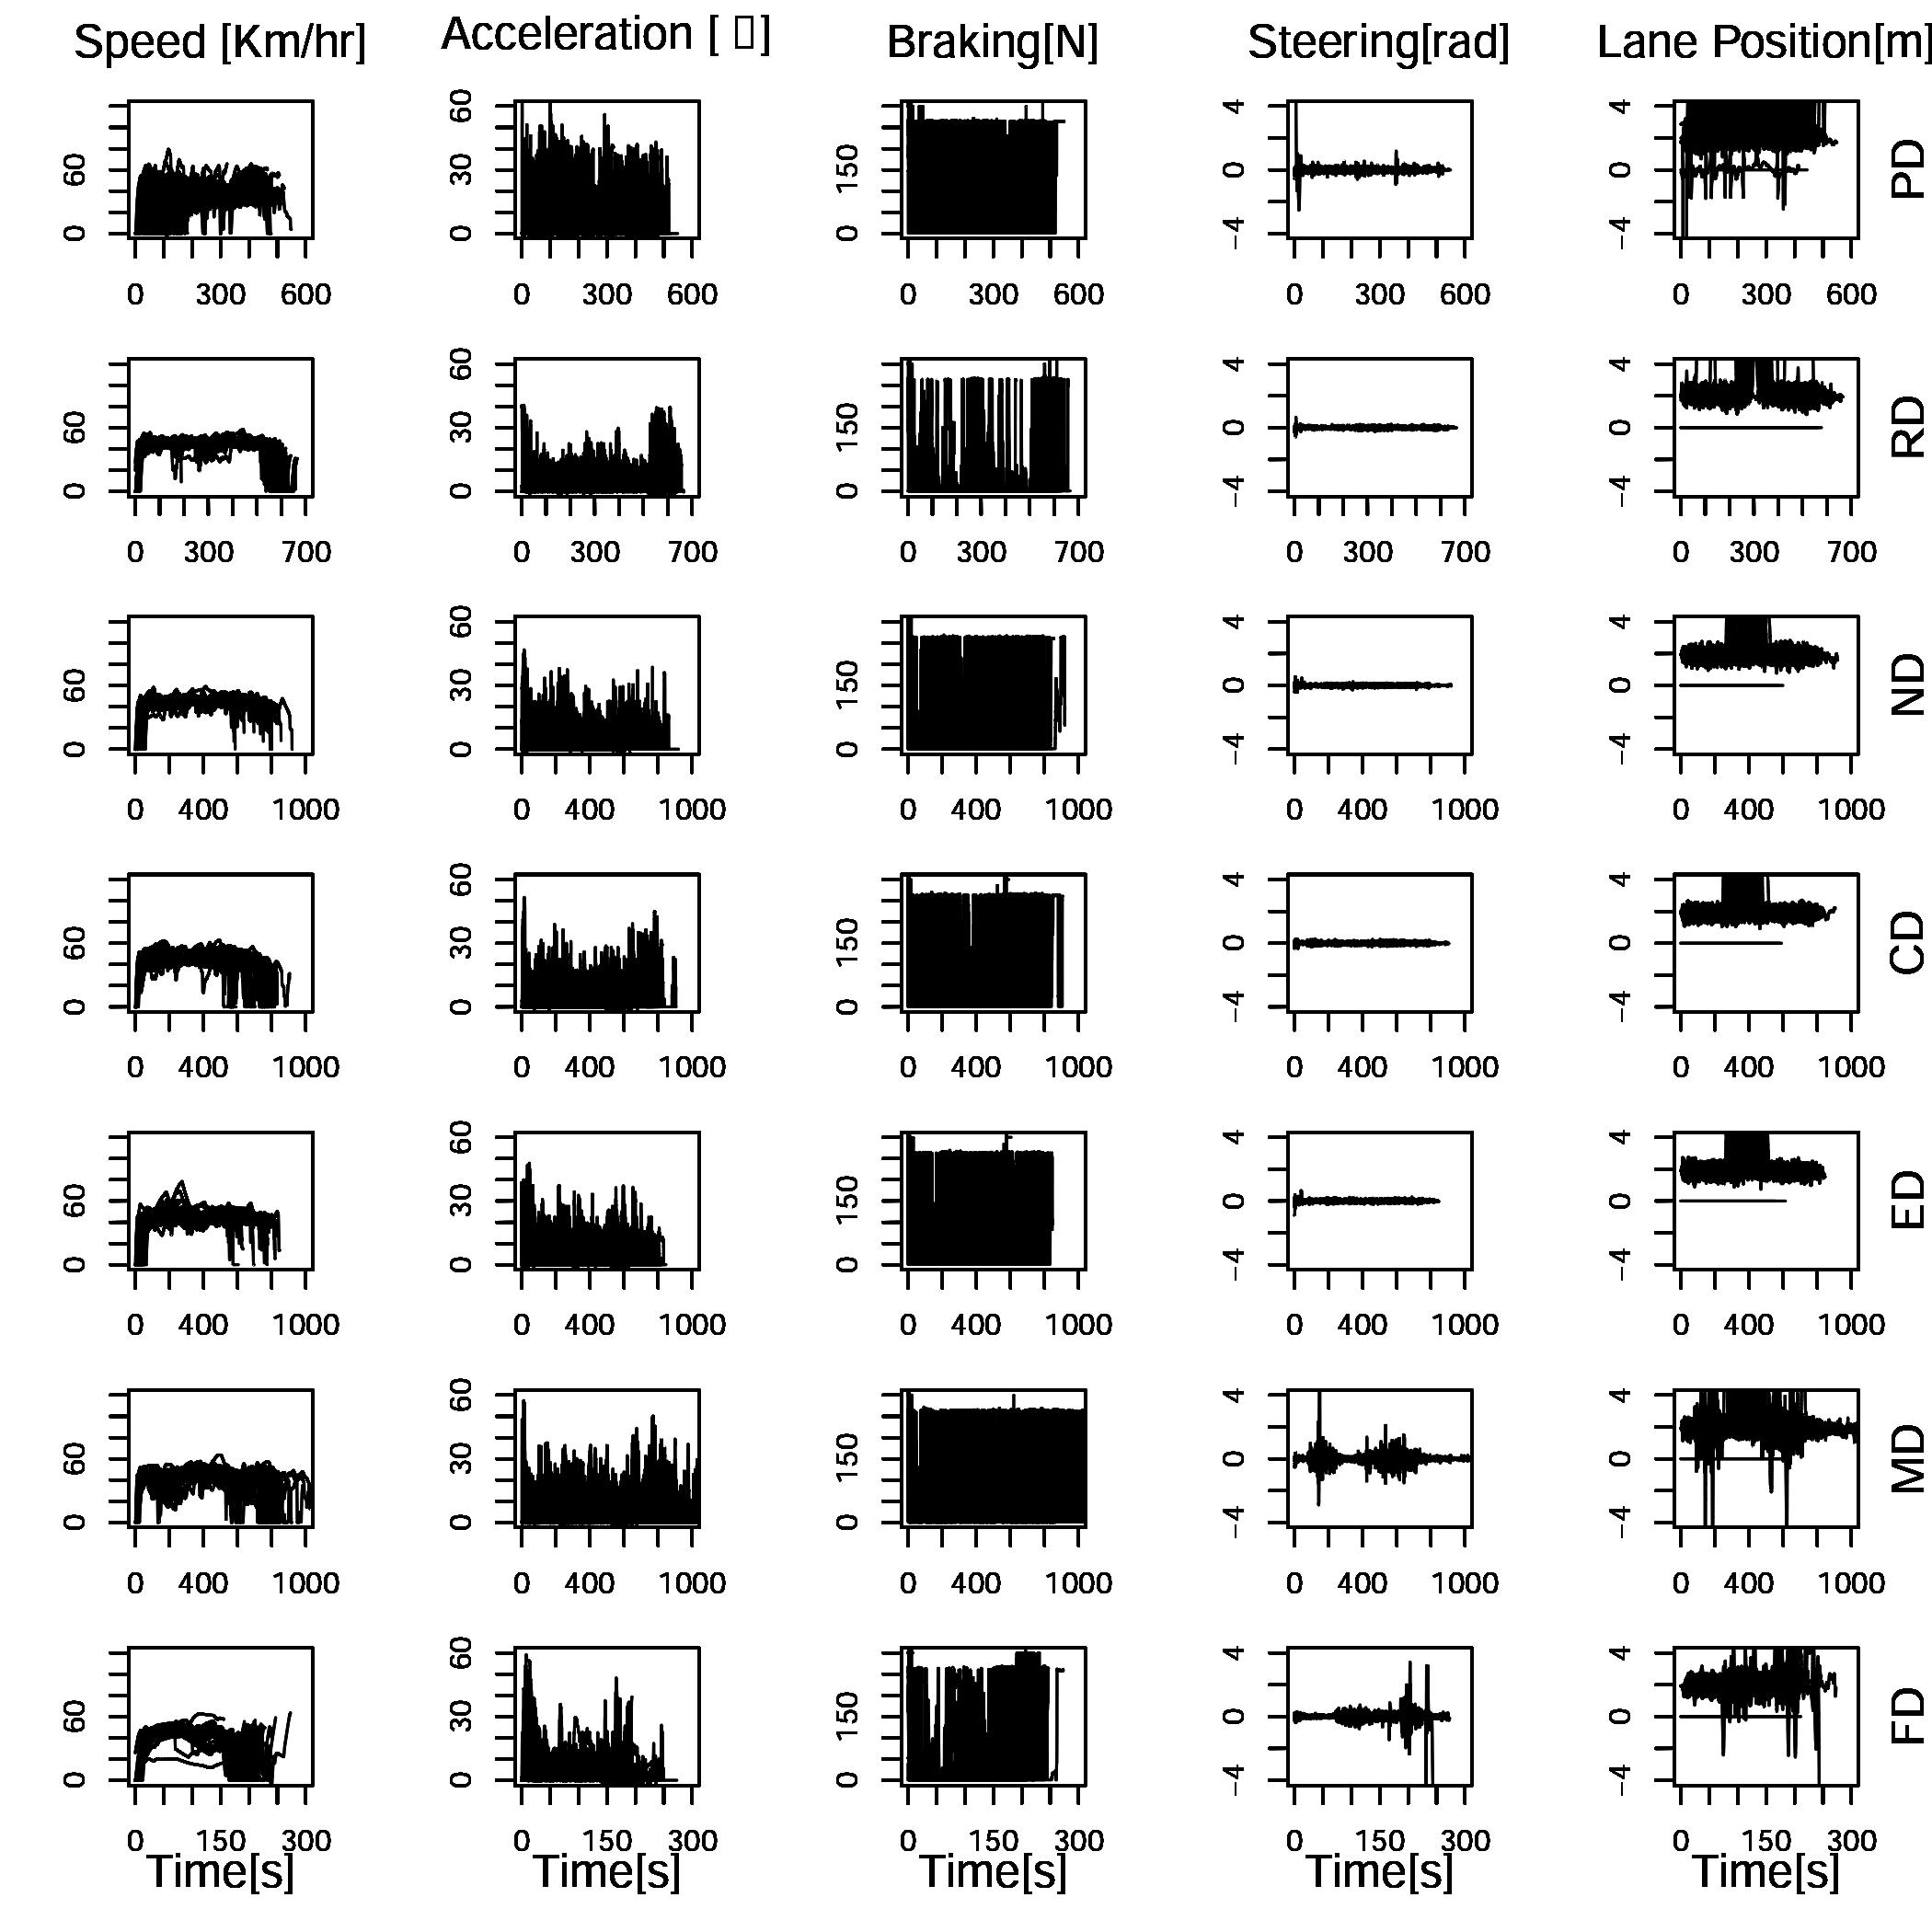
\includegraphics[width=1.0\textwidth]{Res.jpg}
\caption{\label{fig:res}Performance Signals per variable and drive, for all subjects}
\end{figure}
\FloatBarrier




% \subsection{How to add Lists}

% You can make lists with automatic numbering \dots
% href{https://www.overleaf.com/blog/184}{Mendeley}, CiteULike or Zotero library as a \verb|.bib| file. You can then cite entries from it, like this: \cite{greenwade93}. Just remember to specify a bibliography style, as well as the filename of the \verb|.bib|.

% You can find a \href{https://www.overleaf.com/help/97-how-to-include-a-bibliography-using-bibtex}{video tutorial here} to learn more about BibTeX.

% We hope you find Overleaf useful, and please let us know if you have any feedback using the help menu above --- or use the contact form at \url{https://www.overleaf.com/contact}!

% \bibliographystyle{alpha}
% \bibliography{sample}

\end{document}